\documentclass[a4paper,11pt,abstracton,hidelinks]{scrartcl}
\usepackage{dphil}
\usepackage{wasysym}
\addbibresource{refs.bib}
% hide section numbers
\setcounter{secnumdepth}{0}


\title{
Chapter 3. The \textit{Anopheles gambiae} 1000 Genomes Project phase 1 nucleotide variation data resource
}


\author{}


\begin{document}
\renewcommand{\abstractname}{Summary}


\maketitle



%%%%%%%%%%%%%%%%%%%%%%%%%%%%%%%%%%%%%%%%%%%%%%%%%%%%%%%%%%%%%%%%%%%%%%%%%%%%%%%
%%%%%%%%%%%%%%%%%%%%%%%%%%%%%%%%%%%%%%%%%%%%%%%%%%%%%%%%%%%%%%%%%%%%%%%%%%%%%%%
%%%%%%%%%%%%%%%%%%%%%%%%%%%%%%%%%%%%%%%%%%%%%%%%%%%%%%%%%%%%%%%%%%%%%%%%%%%%%%%
\begin{abstract}


In this chapter I describe the production and curation of a data resource of nucleotide variation obtained from whole-genome sequencing of 888 individual mosquitoes wild-caught from natural populations and a further 80 individuals from colony crosses.
%
Production of this data resource was a collaborative effort involving members of multiple research teams within the Ag1000G Consortium.
%
My contribution, described in this chapter, was to analyse the raw variant calls, define and carry out quality control and validation analyses, investigate genome accessibility and define quality filters, and produce the final analysis-ready data resource.
%
I also report analyses of these data to quantify the levels of nucleotide variation found, and to explore how genomic features such as protein-coding genes affect the genomic landscape of nucleotide variation.


\end{abstract}


\tableofcontents


%%%%%%%%%%%%%%%%%%%%%%%%%%%%%%%%%%%%%%%%%%%%%%%%%%%%%%%%%%%%%%%%%%%%%%%%%%%%%%%
%%%%%%%%%%%%%%%%%%%%%%%%%%%%%%%%%%%%%%%%%%%%%%%%%%%%%%%%%%%%%%%%%%%%%%%%%%%%%%%
%%%%%%%%%%%%%%%%%%%%%%%%%%%%%%%%%%%%%%%%%%%%%%%%%%%%%%%%%%%%%%%%%%%%%%%%%%%%%%%
\section{Introduction}


As described in chapter 1, the Ag1000G Project aims to use whole-genome deep Illumina sequencing to explore natural genetic variation among populations of malaria vectors within the \textit{An. gambiae} complex.
%
For logistical reasons the project was divided into three phases, and a total of 888 mosquito specimens sampled from natural populations were included in the first project phase.
%
A further 80 mosquito specimens comprising parents and progeny of four colony crosses were also sequenced within this project phase.
%
This chapter is primarily methodological, describing the processes and analyses developed and used to identify, genotype and validate single nucleotide polymorphisms (SNPs) among these specimens.
%
For completeness, I have included some brief methodological information regarding population sampling and whole-genome sequencing which were performed by members of the Ag1000G Consortium.
%
However, the main focus of this chapter is the work I contributed to production and validation of a high quality genome-wide resource of SNP data from sequencing of these specimens.
%
Where work was carried out by or in collaboration with other members of the Ag1000G Consortium I have indicated that within the relevant subsection.



%%%%%%%%%%%%%%%%%%%%%%%%%%%%%%%%%%%%%%%%%%%%%%%%%%%%%%%%%%%%%%%%%%%%%%%%%%%%%%%
%%%%%%%%%%%%%%%%%%%%%%%%%%%%%%%%%%%%%%%%%%%%%%%%%%%%%%%%%%%%%%%%%%%%%%%%%%%%%%%
%%%%%%%%%%%%%%%%%%%%%%%%%%%%%%%%%%%%%%%%%%%%%%%%%%%%%%%%%%%%%%%%%%%%%%%%%%%%%%%
\section{Methods}


%%%%%%%%%%%%%%%%%%%%%%%%%%%%%%%%%%%%%%%%%%%%%%%%%%%%%%%%%%%%%%%%%%%%%%%%%%%%%%%
%%%%%%%%%%%%%%%%%%%%%%%%%%%%%%%%%%%%%%%%%%%%%%%%%%%%%%%%%%%%%%%%%%%%%%%%%%%%%%%
\subsection{Population sampling}


\begin{figure}[t!]
\centering
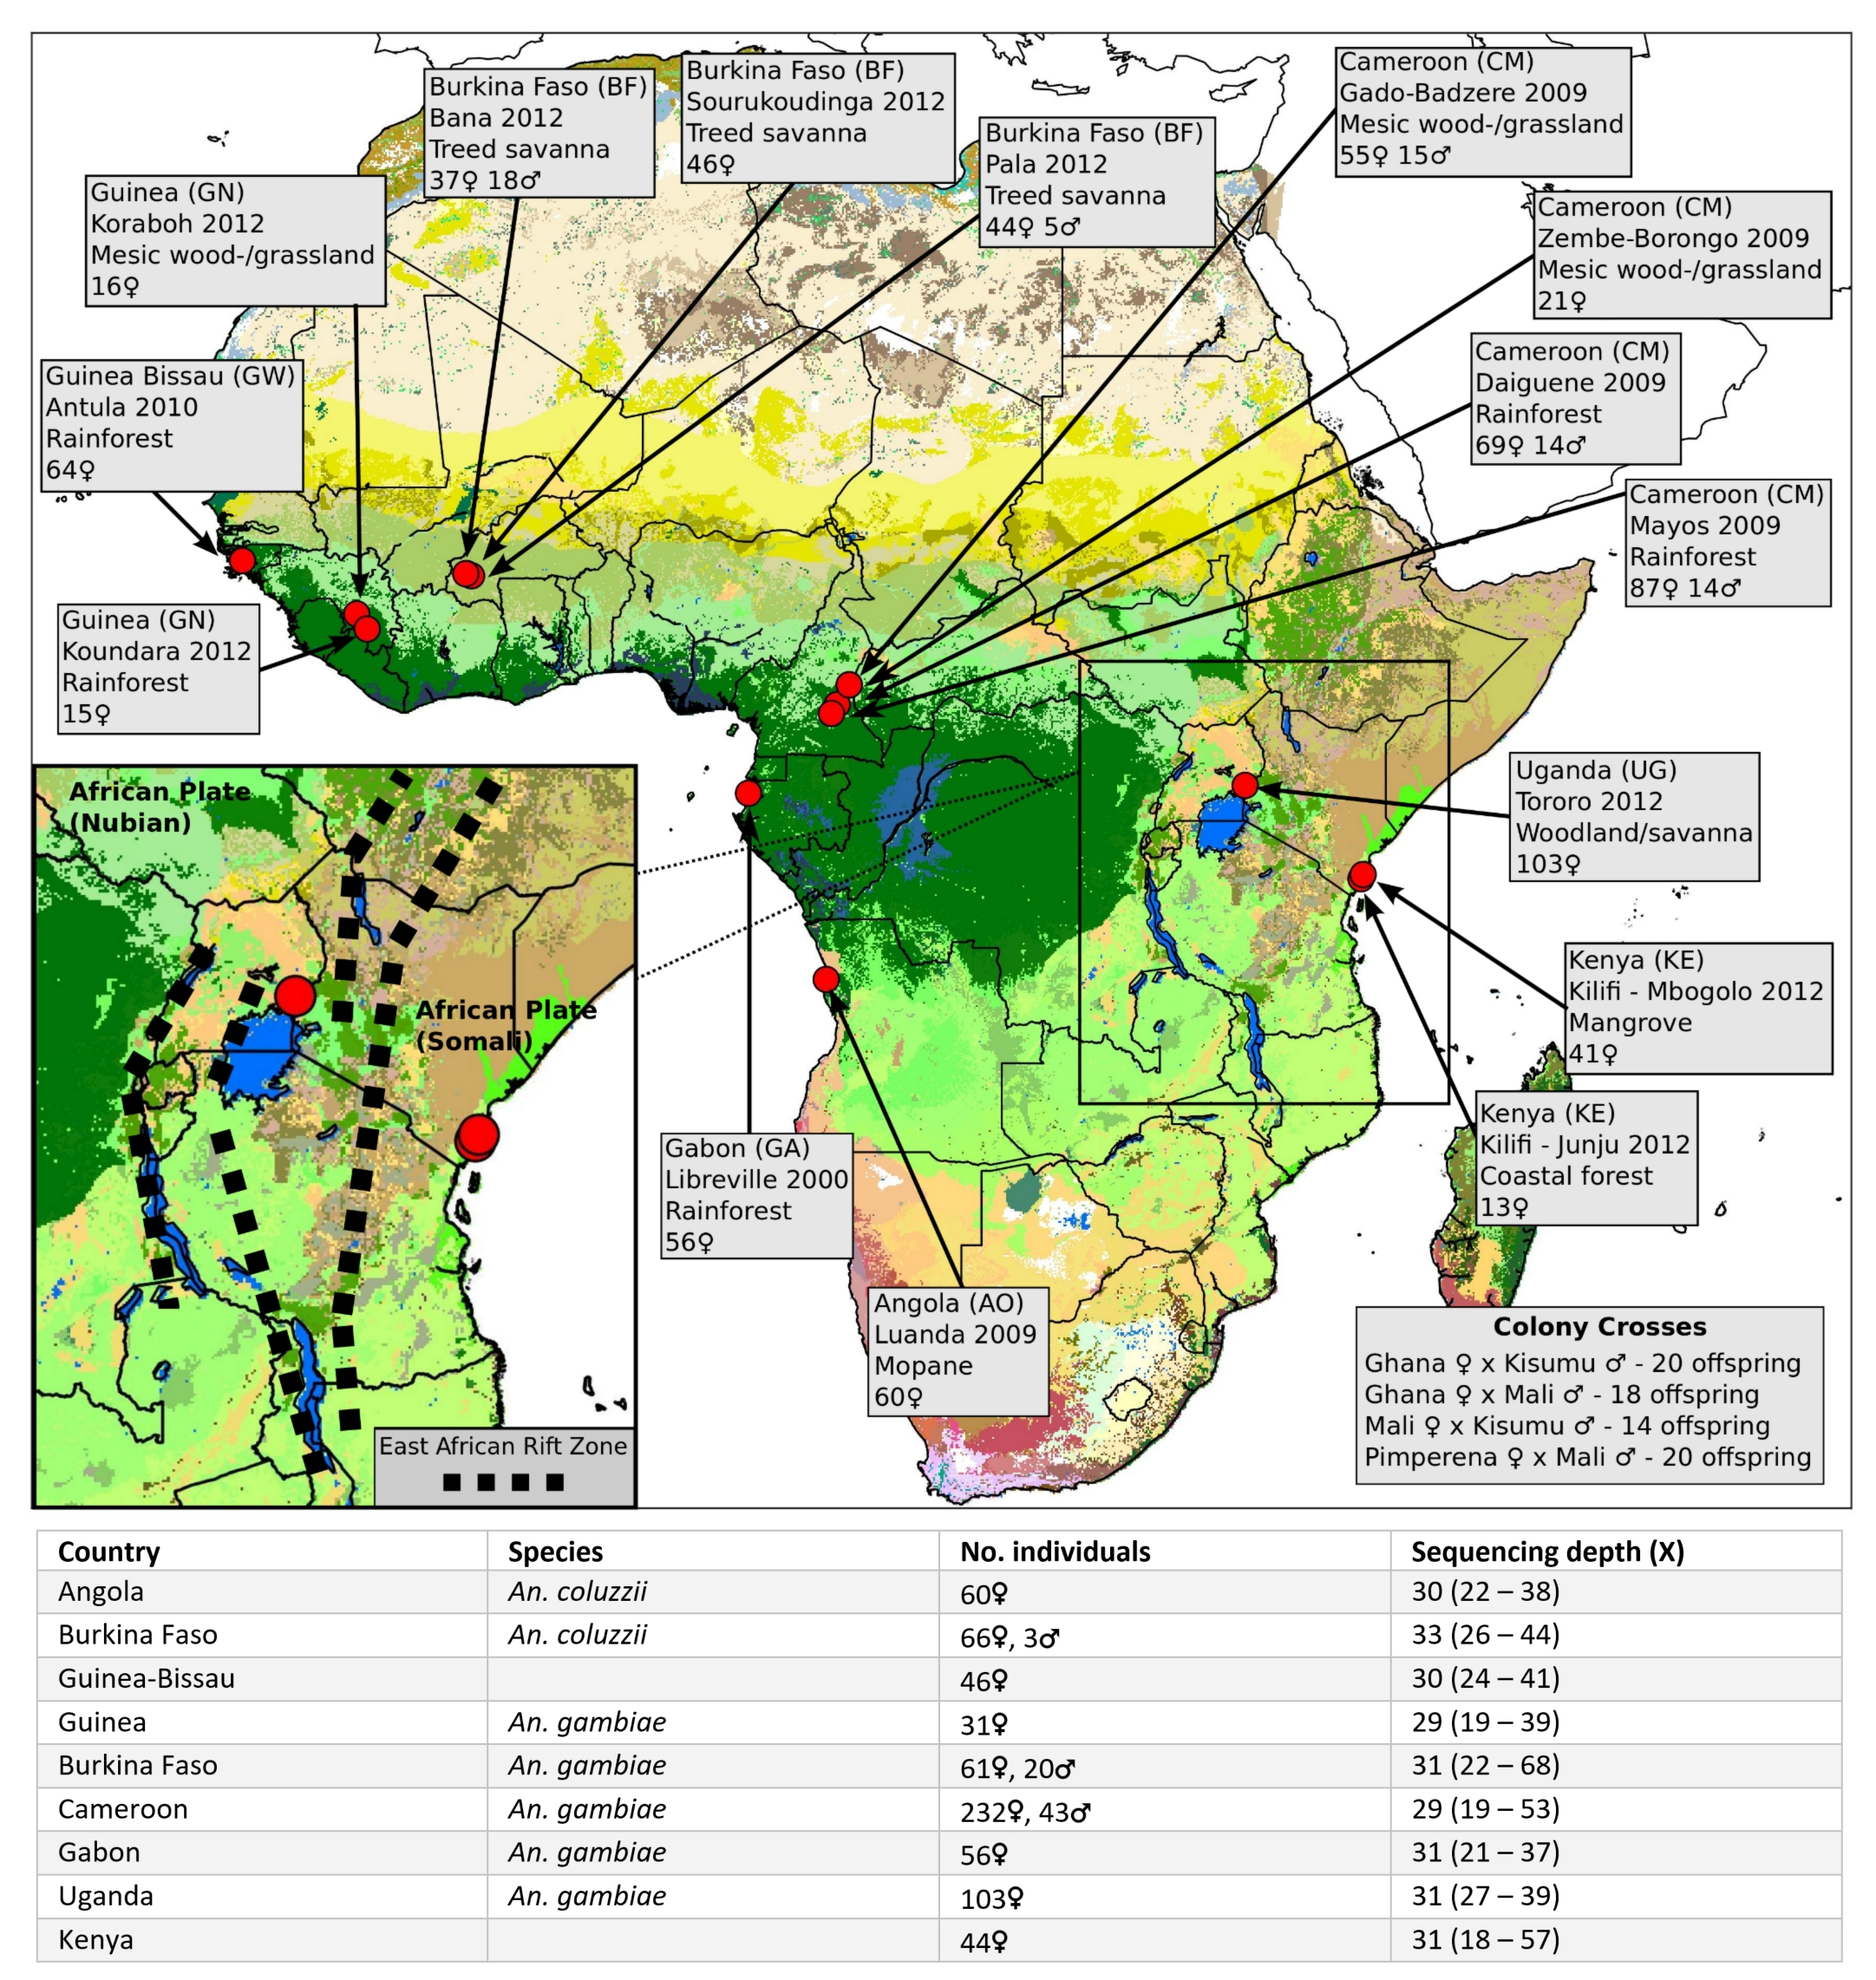
\includegraphics[width=\textwidth]{artwork/chapter3/map.jpeg}
\caption{Map of sampling locations.
%
Numbers of specimens are shown by gender.
%
Parental colonies and numbers of offspring for colony crosses are shown inset.
%
Numbers of samples are shown after removing samples that failed any of the quality control steps described in this chapter. 
%
Colours in the map denote ecosystem classes, see \citet{Sayre2013} Fig. 9 for a complete colour legend. 
%
This figure was produced in collaboration with Chris Clarkson.}
\label{fig:map}
\end{figure}


\textit{Population sampling was performed by members of the Ag1000G Consortium. Below is a brief description of the cohort of mosquito specimens obtained for sequencing. A more detailed description is available in \citet{Ag1000G2017}.}


%%
A total of 888 mosquito specimens collected from natural populations were included in the Ag1000G phase 1 cohort.
%
This included mosquitoes representing two major malaria vector species  \textit{An. gambiae} and \textit{An. coluzzii}.
%
Mosquitoes were sampled from 8 countries in sub-Saharan Africa representing a broad geographical range spanning the continent: Guinea-Bissau, Guinea, Burkina Faso, Cameroon, Gabon, Angola, Uganda and Kenya (Fig. \ref{fig:map}).
%
Mosquitoes had been collected prior to the initiation of the Ag1000G Project as part of previous field studies, and were collected at different times, with the earliest collections being in 2000 (Gabon) and the most recent in 2012 (Burkina Faso).
%
Because these mosquitoes were collected in the context of different studies, a number of different collection methods were used, including light traps, pyrethrum spray catch and larval collection.
%
In addition to the wild-caught specimens, a further 80 mosquitoes were obtained from four colony crosses, each cross comprising two parents and up to 20 progeny, where parents were drawn from established reference colonies (Fig. \ref{fig:map} inset).
%
The main rationale for including colony crosses was to provide a mechanism for calibrating and measuring the accuracy of variant calling methods, because colony crosses allow for the analysis of genetic inheritance and Mendelian inconsistencies between parents and offspring, which can be a useful proxy of variant calling errors \citep{Saunders2007,Pilipenko2014}.
%
DNA extraction was performed on individual mosquitoes and genomic DNA samples were shipped to the Wellcome Sanger Institute for sequencing.


%%%%%%%%%%%%%%%%%%%%%%%%%%%%%%%%%%%%%%%%%%%%%%%%%%%%%%%%%%%%%%%%%%%%%%%%%%%%%%%
%%%%%%%%%%%%%%%%%%%%%%%%%%%%%%%%%%%%%%%%%%%%%%%%%%%%%%%%%%%%%%%%%%%%%%%%%%%%%%%
\subsection{Whole-genome sequencing}


\textit{Whole-genome sequencing was performed by staff at the MalariaGEN Resource Center and the Wellcome Sanger Institute sample logistics, sequencing and informatics facilities. Below is a brief description of sequencing methods. A more detailed description is available in \citet{Ag1000G2017}.}


%%
Sequencing was performed on the Illumina HiSeq 2000 platform at the Wellcome Sanger Institute.
%
Paired-end multiplex libraries were prepared using the manufacturer's protocol, with the exception that genomic DNA was fragmented using Covaris Adaptive Focused Acoustics rather than nebulization.
%
Multiplexes comprised 12 tagged individual mosquitoes and three lanes of sequencing were generated for each multiplex to even out variations in yield between sequencing runs.
%
Thus after sequencing data were demultiplexed, data for each individual sample were available from three separate sequencing runs.
%
Cluster generation and sequencing were undertaken per the manufacturer's protocol for paired-end 100 bp sequence reads with insert size in the range 100-200 bp.
%
Target coverage was $30\times$ per individual.
%
The median depth of coverage obtained per individual was at least $29\times$ for all of the sample sets contributed (Table \ref{table:coverage}).
%

\begin{table}[t]

\begin{center}

\begin{threeparttable}

\caption{Depth of coverage.
Coverage column shows median (interquartile range) depth coverage for all samples by country and species.
%
Numbers of samples and coverage values are shown after removing samples that failed any of the quality control steps described in this chapter. 
%
Species status is uncertain for samples from Guinea-Bissau and Kenya, see Chapter 4 for further explanation.
}

\label{table:coverage}

\begin{tabular}{llll}
 \hline
 \textbf{Country} & \textbf{Species} & \textbf{No. samples} (\female, \male) & \textbf{Coverage} \\
 \hline
 Angola & \textit{An. coluzzii} & 60, 0 & 30 (22-38) \\
 Burkina Faso & \textit{An. coluzzii} & 66, 3 & 33 (26-44) \\
 Burkina Faso & \textit{An. gambiae} & 61, 20 & 31 (22-68) \\
 Cameroon & \textit{An gambiae} & 232, 43 & 29 (19-53) \\
 Gabon & \textit{An. gambiae} & 56, 0 & 31 (21-37) \\
 Guinea & \textit{An. gambiae} & 31, 0 & 29 (19-39) \\
 Uganda & \textit{An. gambiae} & 103, 0 & 31 (27-39) \\
 Guinea Bissau & uncertain & 46, 0 & 30 (24-41) \\
 Kenya & uncertain & 44, 0 & 31 (18-57) \\
 \hline
\end{tabular}

\end{threeparttable}

\end{center}

\end{table}


%%%%%%%%%%%%%%%%%%%%%%%%%%%%%%%%%%%%%%%%%%%%%%%%%%%%%%%%%%%%%%%%%%%%%%%%%%%%%%%
%%%%%%%%%%%%%%%%%%%%%%%%%%%%%%%%%%%%%%%%%%%%%%%%%%%%%%%%%%%%%%%%%%%%%%%%%%%%%%%
\subsection{SNP discovery and genotyping}


\textit{SNP discovery and genotyping was performed in collaboration with the MalariaGEN Resource Center data production team. Below is a brief description of SNP calling methods. A more detailed description is available in \citet{Ag1000G2017}.}


%%
SNP discovery and genotyping was formed following best practices defined for the Genome Analysis Toolkit (GATK) version 2 \citep{McKenna2010,Depristo2011,VanderAuwera2013}.
%
Sequence reads from each sample were aligned to the AgamP3 reference genome \citep{Holt2002,Sharakhova2007} using BWA version 0.6.2 \citep{Li2009} using the \textit{aln} and \textit{sampe} commands.
%
A BAM file for each individual was constructed by merging alignments from multiple lanes, and duplicate reads were marked using Picard version 1.96.
%
Reads were then re-aligned around putative indels found within the alignments using GATK.
%
SNP discovery and genotyping was performed using GATK \textit{UnifiedGenotyper}.
%
\textit{UnifiedGenotyper} was run within non-overlapping 10 kb chunks and the results combined into a single variant call format (VCF) file for each chromosome arm using the \textit{vcf-concat} command from vcftools version 0.1.10.
%
SNP discovery was performed using the 888 wild-caught samples.
%
The colony crosses samples were then genotyped at the same set of SNPs using GATK \textit{UnifiedGenotyper}.


%%%%%%%%%%%%%%%%%%%%%%%%%%%%%%%%%%%%%%%%%%%%%%%%%%%%%%%%%%%%%%%%%%%%%%%%%%%%%%%
%%%%%%%%%%%%%%%%%%%%%%%%%%%%%%%%%%%%%%%%%%%%%%%%%%%%%%%%%%%%%%%%%%%%%%%%%%%%%%%
\subsection{Sample quality control}


%
A number of issues can arise in the process of sample and library preparation and high-throughput sequencing which result in data of insufficient quality to perform robust variant discovery and genotyping.
%
These issues include:
%
\begin{itemize}
%
\item \textbf{Low yield.} The number of sequence reads generated for and individual sample is not sufficient to achieve the desired depth of coverage.
%
\item \textbf{Low library complexity.} If the input DNA quantity is insufficient, the DNA amplification process can generate sufficient material for sequencing, but there may be significant bias, in the sense that some genome regions are overrepresented and others are underrepresented or not covered at all \citep{Head2018}.
%
\item \textbf{Cross-contamination.} During specimen handling, sample preparation and library preparation, material and thus DNA from one sample may contaminate another. In this case the sequencing data generated will include a mixture of reads from the original sample and the contaminating sample.
%
\item \textbf{Metadata errors.} Errors may arise during the recording and transfer of metadata about specimens and samples between information systems. This can lead to situations where the identity of one sample becomes swapped with that of another sample.
%
\item \textbf{Unexpected taxa.} In Ag1000G phase 1 only \textit{An. gambiae} and \textit{An. coluzzii} mosquitoes were to be included. However, not all specimens had the conventional diagnostic species assays performed prior to selection, and thus were only identified morphologically.
\end{itemize}
%
In this subsection I describe analyses performed to identify and exclude samples affected by one or more of these issues.


%%%%%%%%%%%%%%%%%%%%%%%%%%%%%%%%%%%%%%%%%%%%%%%%%%%%%%%%%%%%%%%%%%%%%%%%%%%%%%%
\subsubsection{Sequencing data quality}


\begin{figure}[t!]
\centering
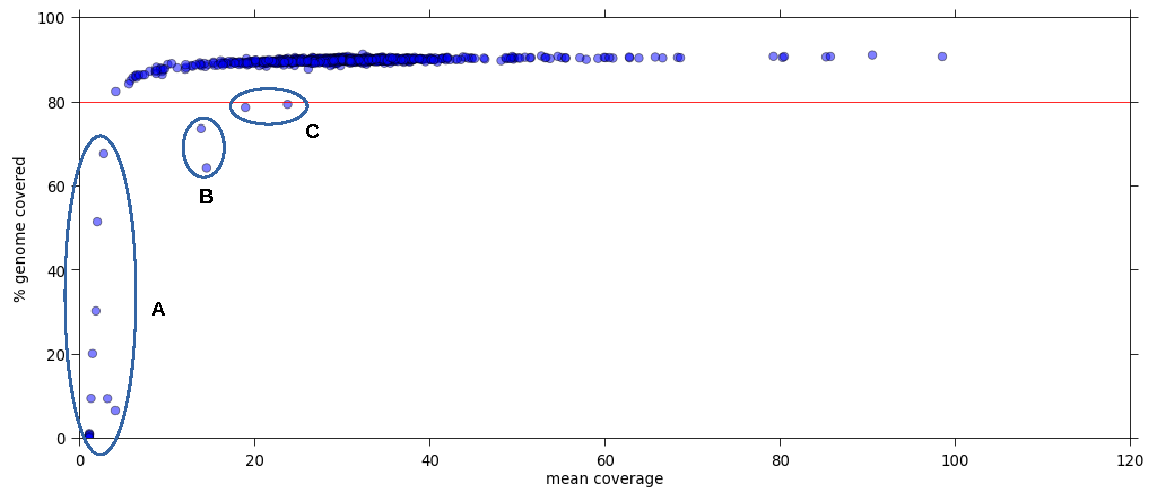
\includegraphics[width=\textwidth]{artwork/chapter3/coverage.pdf}
\caption{Sequencing data quality diagnostics.
%
Each marker represents an individual sample.
%
Mean coverage is computed as total number of sequenced bases divided by genome size.
%
Percent genome covered is percent of nucleotides in reference genome with at least one read aligned.
%
Highlighted groups A, B and C indicate different quality issues, described in the text.
}
%
\label{fig:coverage}
\end{figure}


%%
I analysed summary statistics generated from the sequence read alignments to identify samples with sequencing data quality issues such as low yield or low library complexity.
%
These statistics included the number of sequence reads, mean coverage, percentage of reads mapped tro the reference genome, percentage of reads marked as duplicates, and percentage of aligned bases mismatching the reference genome.
%
I plotted various combinations of these statistics to investigate their distributions and identify outliers.
%
A particularly informative plot was to compare the mean coverage and the percentage of genome covered by at least one read (Fig. \ref{fig:coverage}).
%
Most samples obtained greater than 80\% of the genome covered, but a set of 13 samples had both mean coverage below $7\times$ and less than 80\% of the genome covered, indicating insufficient coverage due to low sequencing yield (Fig. \ref{fig:coverage} group A).
%
There were also four samples with high mean coverage but less than 80\% genome covered.
%
Two of these samples had a high rate of duplicate reads, and thus poor genome coverage was likely due to low library complexity (Fig. \ref{fig:coverage} group B).
%
The remaining two samples had a higher mismatch rate, thus poor genome coverage was likely due to an unexpected taxon with higher divergence from the reference genome (Fig. \ref{fig:coverage} group C).
%
On the basis of these analyses, the percentage of genome covered appeared to be a useful metric capturing multiple quality issues, and I excluded 17 samples with less than 80\% genome covered.
%


%%%%%%%%%%%%%%%%%%%%%%%%%%%%%%%%%%%%%%%%%%%%%%%%%%%%%%%%%%%%%%%%%%%%%%%%%%%%%%%
\subsubsection{Cross-contamination}


\begin{figure}[t!]
\centering
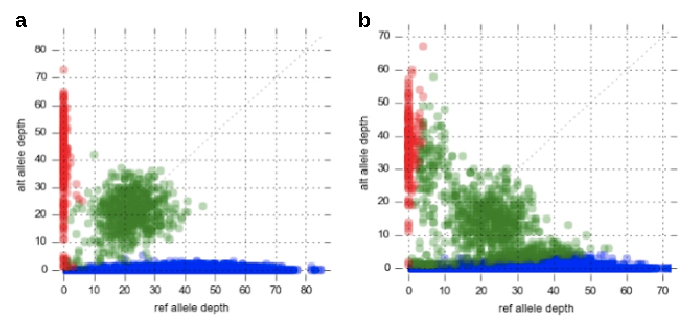
\includegraphics[width=\textwidth]{artwork/chapter3/contamination.pdf}
\caption{Cross-contamination diagnostics.
%
Each plot shows an allele balance diagnostic plot for a single sample.
%
Each marker within a plot is a genotype call (blue = homozygous reference; green = heterozygous; red = homozygous alternate).
%
\textbf{a}, Example of sample with predicted contamination $<2\%$.
%
\textbf{b}, Example of sample with predicted contamination $>4\%$.
}
%
\label{fig:contamination}
\end{figure}


%%
Cross-contamination between samples of the same species can be detected by analysing the fractions of reads supporting genotypes in each sample.
%
Several tools have been developed to detect cross-contamination in sequencing data, such as verifyBamID \citep{Jun2012}.
%
Previous human sequencing projects have used verifyBamID and excluded samples with an estimated contamination fraction above 2\% \citep{1000G2015}.
%
To analyse evidence for cross-contamination in the Ag1000G phase 1 samples, verifyBamID was run on all samples by the MalariaGEN data production team.
%
Because this tool had been developed for and previously only applied in human sequencing studies, I performed additional analyses to confirm that the contamination predictions were reliable in \textit{Anopheles}.
%
I generated a set of diagnostic allele balance plots for each of the 888 mosquito samples in phase 1 which plotted data from genotypes across all autosomes, showing the genotype called and the numbers of reads supporting the reference and alternate alleles (e.g., Fig. \ref{fig:contamination}). 
%
I then visually inspected these plots and cross-referenced them against the contamination fraction predicted by verifyBamID.
%
In uncontaminated samples there was clear separation between the different possible genotype calls (e.g., Fig. \ref{fig:contamination}a) and cases of contamination were evident as a lack of a clear separation between genotype calls (e.g., Fig. \ref{fig:contamination}b).
%
In all cases where verifyBamID predicted contamination $>4\%$ I confirmed a signal of contamination via allele balance plots, and conversely I found no cases of allele balance plots indicating contamination but verifyBamID predicted contamination $<4\%$, providing confidence that verifyBamID predictions were reliable. 
%
To be conservative, I excluded all samples with verifyBamID contamination $>2\%$ from the final dataset.
%


%%%%%%%%%%%%%%%%%%%%%%%%%%%%%%%%%%%%%%%%%%%%%%%%%%%%%%%%%%%%%%%%%%%%%%%%%%%%%%%
\subsubsection{Sex metadata concordance}


\begin{figure}[t!]
\centering
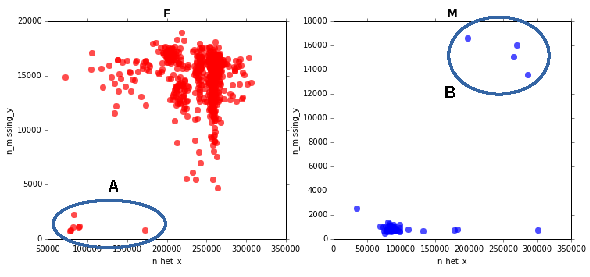
\includegraphics[width=\textwidth]{artwork/chapter3/sex.pdf}
\caption{Sex metadata concordance checks.
%
Each marker represents a sample.
%
The left panel shows samples from mosquitoes reported in metadata as female, the right panel shows samples reported as male.
%
$n\_het\_x$ = No. of heterozygous genotype calls on the $X$ chromosome.
%
$n\_missing\_y$ = No. of missing genotype calls on the $Y\_unplaced$ chromosome.
%
Groups labelled A and B are described in the text.
%
}
%
\label{fig:sex}
\end{figure}


%%
Both male and female mosquito specimens were contributed to Ag1000G phase 1 (Table \ref{table:coverage}) and the morphologically-identified gender was included in the sample metadata contributed by the Ag1000G consortium partners who collected the specimens.
%
To confirm metadata records were correct, I compared the reported specimen gender with a gender call made directly from the sequencing data.
%
To call gender for each sample I computed the counts of homozygous, heterozygous and missing genotype calls separately for the X and Y chromosomes. 
%
Sex determination is similar in mosquitoes to humans in that females are homogametic XX and males are heterogametic XY.
%
Thus in females we expect to observe heterozygous genotype calls on the X chromosome and missing genotype calls on the Y chromosome.
%
Conversely in males we expect only homozygous genotype calls on the X chromosome and non-missing genotype calls on the Y chromosome.
%
Plotting these data it was evident that some samples had genotype counts not consistent with their reported sex (Fig. \ref{fig:sex}).
%
This included six samples reported as female but with male genotype counts (Fig. \ref{fig:sex} group A) and four samples reported as male but with female genotype counts (Fig. \ref{fig:sex} group B).
%
I excluded these ten samples from further analyses.
%
There were also a further six samples with apparently androgenous genotype counts on sex chromosomes.
%
Cross-checking against the contamination analysis showed these apparently androgenous samples to have predicted contamination $>2\%$, explaining the unusual sex chromosome genotype counts.
%%


%%%%%%%%%%%%%%%%%%%%%%%%%%%%%%%%%%%%%%%%%%%%%%%%%%%%%%%%%%%%%%%%%%%%%%%%%%%%%%%
\subsubsection{Population outliers}


@@TODO


%%%%%%%%%%%%%%%%%%%%%%%%%%%%%%%%%%%%%%%%%%%%%%%%%%%%%%%%%%%%%%%%%%%%%%%%%%%%%%%
\subsubsection{Minimum depth of coverage}


@@TODO


%%%%%%%%%%%%%%%%%%%%%%%%%%%%%%%%%%%%%%%%%%%%%%%%%%%%%%%%%%%%%%%%%%%%%%%%%%%%%%%
\subsection{Variant quality control}


@@TODO



%%%%%%%%%%%%%%%%%%%%%%%%%%%%%%%%%%%%%%%%%%%%%%%%%%%%%%%%%%%%%%%%%%%%%%%%%%%%%%%
\subsubsection{Genome accessibility}


@@TODO


%%%%%%%%%%%%%%%%%%%%%%%%%%%%%%%%%%%%%%%%%%%%%%%%%%%%%%%%%%%%%%%%%%%%%%%%%%%%%%%
\subsubsection{Variant filters}


@@TODO


%%%%%%%%%%%%%%%%%%%%%%%%%%%%%%%%%%%%%%%%%%%%%%%%%%%%%%%%%%%%%%%%%%%%%%%%%%%%%%%
%%%%%%%%%%%%%%%%%%%%%%%%%%%%%%%%%%%%%%%%%%%%%%%%%%%%%%%%%%%%%%%%%%%%%%%%%%%%%%%
\subsection{Production of the analysis-ready genome variation dataset}


@@TODO


%%%%%%%%%%%%%%%%%%%%%%%%%%%%%%%%%%%%%%%%%%%%%%%%%%%%%%%%%%%%%%%%%%%%%%%%%%%%%%%
%%%%%%%%%%%%%%%%%%%%%%%%%%%%%%%%%%%%%%%%%%%%%%%%%%%%%%%%%%%%%%%%%%%%%%%%%%%%%%%
\subsection{Validation with Sanger sequencing}


@@TODO



%%%%%%%%%%%%%%%%%%%%%%%%%%%%%%%%%%%%%%%%%%%%%%%%%%%%%%%%%%%%%%%%%%%%%%%%%%%%%%%
%%%%%%%%%%%%%%%%%%%%%%%%%%%%%%%%%%%%%%%%%%%%%%%%%%%%%%%%%%%%%%%%%%%%%%%%%%%%%%%
%%%%%%%%%%%%%%%%%%%%%%%%%%%%%%%%%%%%%%%%%%%%%%%%%%%%%%%%%%%%%%%%%%%%%%%%%%%%%%%
\section{Results}


@TODO


%%%%%%%%%%%%%%%%%%%%%%%%%%%%%%%%%%%%%%%%%%%%%%%%%%%%%%%%%%%%%%%%%%%%%%%%%%%%%%%
%%%%%%%%%%%%%%%%%%%%%%%%%%%%%%%%%%%%%%%%%%%%%%%%%%%%%%%%%%%%%%%%%%%%%%%%%%%%%%%
%%%%%%%%%%%%%%%%%%%%%%%%%%%%%%%%%%%%%%%%%%%%%%%%%%%%%%%%%%%%%%%%%%%%%%%%%%%%%%%
\section{Conclusion}


@TODO


%%%%%%%%%%%%%%%%%%%%%%%%%%%%%%%%%%%%%%%%%%%%%%%%%%%%%%%%%%%%%%%%%%%%%%%%%%%%%%%
%%%%%%%%%%%%%%%%%%%%%%%%%%%%%%%%%%%%%%%%%%%%%%%%%%%%%%%%%%%%%%%%%%%%%%%%%%%%%%%
%%%%%%%%%%%%%%%%%%%%%%%%%%%%%%%%%%%%%%%%%%%%%%%%%%%%%%%%%%%%%%%%%%%%%%%%%%%%%%%
\section{Acknowledgments}


@TODO


\printbibliography


\end{document}
